% Options for packages loaded elsewhere
\PassOptionsToPackage{unicode}{hyperref}
\PassOptionsToPackage{hyphens}{url}
\documentclass[
  ignorenonframetext,
]{beamer}
\newif\ifbibliography
\usepackage{pgfpages}
\setbeamertemplate{caption}[numbered]
\setbeamertemplate{caption label separator}{: }
\setbeamercolor{caption name}{fg=normal text.fg}
\beamertemplatenavigationsymbolsempty
% remove section numbering
\setbeamertemplate{part page}{
  \centering
  \begin{beamercolorbox}[sep=16pt,center]{part title}
    \usebeamerfont{part title}\insertpart\par
  \end{beamercolorbox}
}
\setbeamertemplate{section page}{
  \centering
  \begin{beamercolorbox}[sep=12pt,center]{section title}
    \usebeamerfont{section title}\insertsection\par
  \end{beamercolorbox}
}
\setbeamertemplate{subsection page}{
  \centering
  \begin{beamercolorbox}[sep=8pt,center]{subsection title}
    \usebeamerfont{subsection title}\insertsubsection\par
  \end{beamercolorbox}
}
% Prevent slide breaks in the middle of a paragraph
\widowpenalties 1 10000
\raggedbottom
\AtBeginPart{
  \frame{\partpage}
}
\AtBeginSection{
  \ifbibliography
  \else
    \frame{\sectionpage}
  \fi
}
\AtBeginSubsection{
  \frame{\subsectionpage}
}
\usepackage{iftex}
\ifPDFTeX
  \usepackage[T1]{fontenc}
  \usepackage[utf8]{inputenc}
  \usepackage{textcomp} % provide euro and other symbols
\else % if luatex or xetex
  \usepackage{unicode-math} % this also loads fontspec
  \defaultfontfeatures{Scale=MatchLowercase}
  \defaultfontfeatures[\rmfamily]{Ligatures=TeX,Scale=1}
\fi
\usepackage{lmodern}
\ifPDFTeX\else
  % xetex/luatex font selection
\fi
% Use upquote if available, for straight quotes in verbatim environments
\IfFileExists{upquote.sty}{\usepackage{upquote}}{}
\IfFileExists{microtype.sty}{% use microtype if available
  \usepackage[]{microtype}
  \UseMicrotypeSet[protrusion]{basicmath} % disable protrusion for tt fonts
}{}
\makeatletter
\@ifundefined{KOMAClassName}{% if non-KOMA class
  \IfFileExists{parskip.sty}{%
    \usepackage{parskip}
  }{% else
    \setlength{\parindent}{0pt}
    \setlength{\parskip}{6pt plus 2pt minus 1pt}}
}{% if KOMA class
  \KOMAoptions{parskip=half}}
\makeatother
\usepackage{longtable,booktabs,array}
\usepackage{caption}
\captionsetup[table]{skip=6pt}
\newcounter{none} % for unnumbered tables
\usepackage{calc} % for calculating minipage widths
\usepackage{caption}
% Make caption package work with longtable
\makeatletter
\def\fnum@table{\tablename~\thetable}
\makeatother
\usepackage{graphicx}
\makeatletter
\newsavebox\pandoc@box
\newcommand*\pandocbounded[1]{% scales image to fit in text height/width
  \sbox\pandoc@box{#1}%
  \Gscale@div\@tempa{\textheight}{\dimexpr\ht\pandoc@box+\dp\pandoc@box\relax}%
  \Gscale@div\@tempb{\linewidth}{\wd\pandoc@box}%
  \ifdim\@tempb\p@<\@tempa\p@\let\@tempa\@tempb\fi% select the smaller of both
  \ifdim\@tempa\p@<\p@\scalebox{\@tempa}{\usebox\pandoc@box}%
  \else\usebox{\pandoc@box}%
  \fi%
}
% Set default figure placement to htbp
\def\fps@figure{htbp}
\makeatother
\setlength{\emergencystretch}{3em} % prevent overfull lines
\providecommand{\tightlist}{%
  \setlength{\itemsep}{0pt}\setlength{\parskip}{0pt}}
% Slide layout defaults for warning-clean scientific decks.
\usepackage{etoolbox}
\IfFileExists{xurl.sty}{\usepackage{xurl}}{}
\IfFileExists{seqsplit.sty}{\usepackage{seqsplit}}{\newcommand{\seqsplit}[1]{#1}}
\protected\def\breakseq#1{\seqsplit{#1}}
\protected\def\breaktt#1{\begingroup\ttfamily\seqsplit{#1}\endgroup}
\setlength{\emergencystretch}{6em}
\tolerance=5000
\hbadness=10000
\hfuzz=1pt
\setlength{\tabcolsep}{2pt}
\AtBeginEnvironment{longtable}{\tiny\renewcommand{\arraystretch}{0.86}\setlength{\tabcolsep}{1pt}}
\AtBeginEnvironment{tabular}{\tiny\renewcommand{\arraystretch}{0.86}\setlength{\tabcolsep}{1pt}}

% Natbib and cross-reference fallbacks — slides don't load natbib
% or cleveref, but combined-PDF manuscript prose may emit these
% commands. The fallback renders citations as a bracketed key list
% and cross-references as detokenized labels so slides don't fail on
% undefined control sequences or raw underscores. \providecommand is
% a no-op if packages load later.
\providecommand{\citep}[1]{[#1]}
\providecommand{\citet}[1]{#1}
\providecommand{\citealp}[1]{#1}
\providecommand{\citeauthor}[1]{#1}
\providecommand{\citeyear}[1]{#1}
\providecommand{\cref}[1]{\texttt{\detokenize{#1}}}
\providecommand{\Cref}[1]{\texttt{\detokenize{#1}}}

\newtheorem{proposition}{Proposition}
\newtheorem{hypothesis}{Hypothesis}
\usepackage{bookmark}
\IfFileExists{xurl.sty}{\usepackage{xurl}}{} % add URL line breaks if available
\urlstyle{same}
% fallback for those not using the hyperref driver hyperxmp:
\makeatletter
\@ifundefined{xmpquote}{\newcommand{\xmpquote}[1]{#1}}{}
\makeatother
\hypersetup{
  hidelinks,
  pdfcreator={LaTeX via pandoc}}

\author{\texorpdfstring{}{}}
\date{}

\begin{document}

\section{Temporal-Spatial Taxonomy for Study Design}\label{sec:taxonomy}

\begin{frame}[fragile,allowframebreaks]{Temporal-Spatial Taxonomy for
Study Design}
DigiPPPiP is organized by two primary axes: temporal structure and
spatial configuration. The configured project has 3 temporal modes, 3
spatial configurations, and 9 total modality cells.
\breakseq{[@fig:taxonomy\_matrix]} is the central map of that design space. The
axes intentionally separate relation from infrastructure: two partners
can be relationally engaged while co-present, remote, delayed, or
hybrid, but each cell changes what can be perceived, logged, repaired,
and revisited.

\begin{figure}
\centering
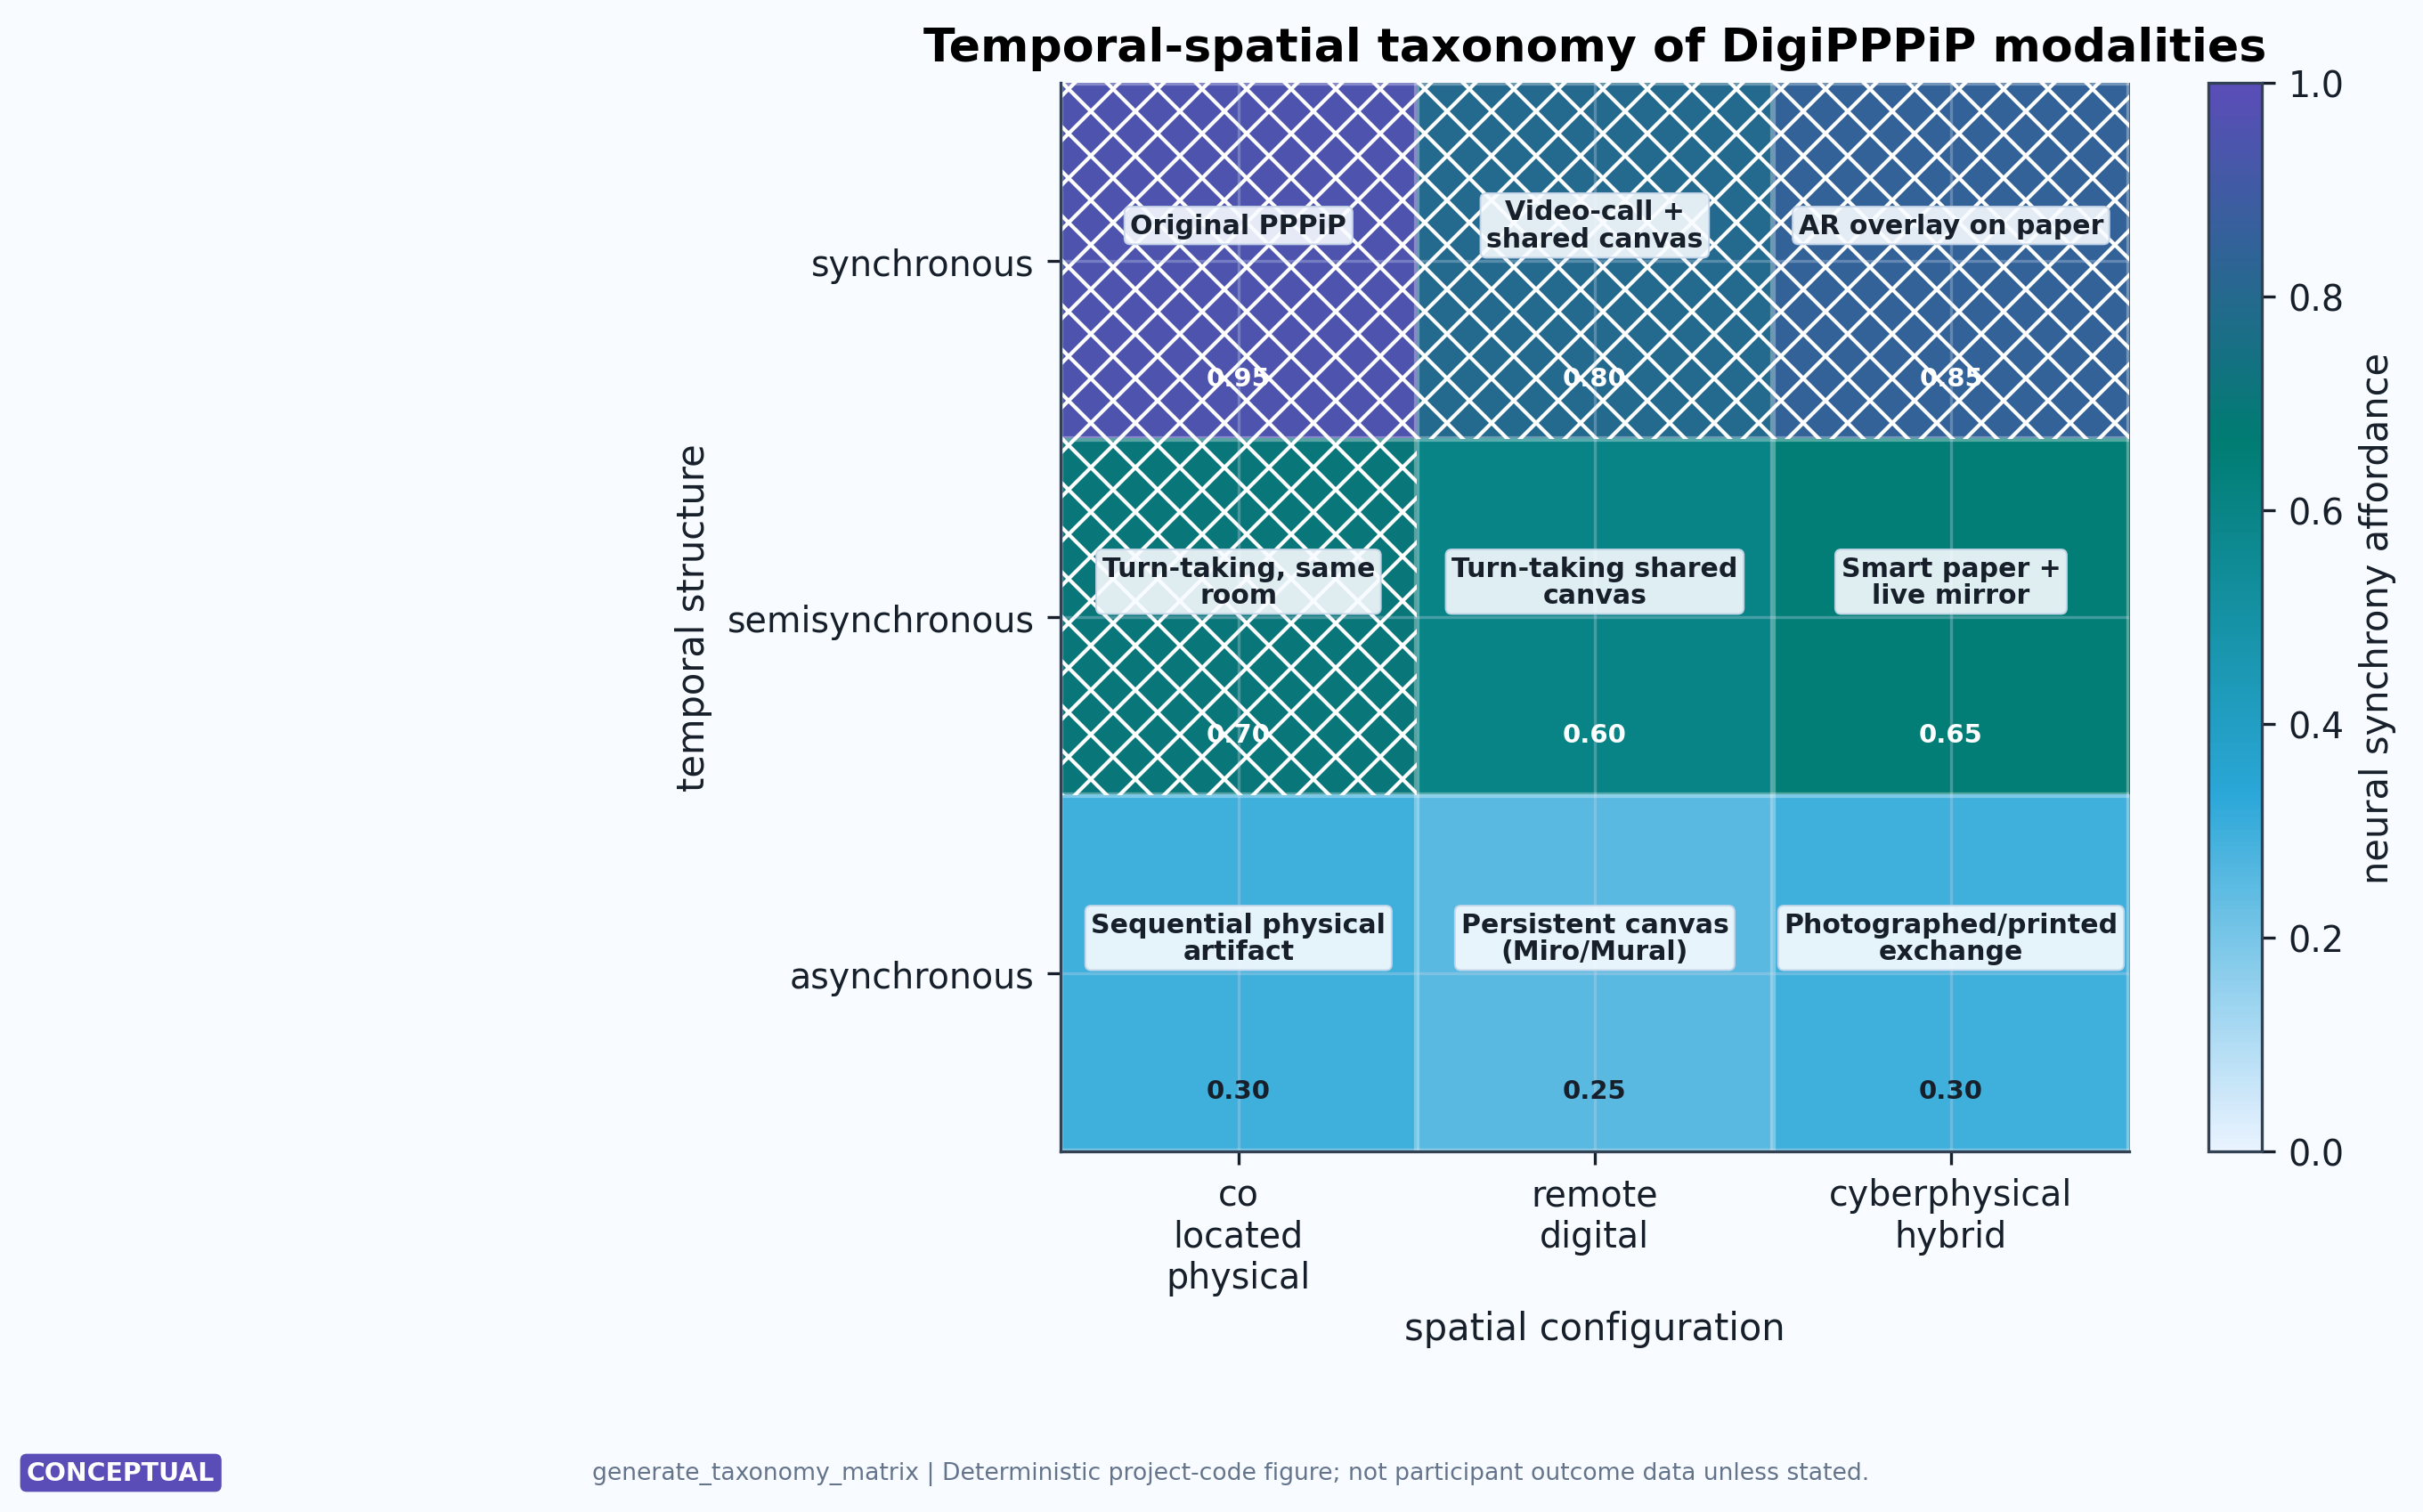
\includegraphics[width=0.9\linewidth,height=0.46\textheight,keepaspectratio,alt={Three-by-three temporal-spatial taxonomy for DigiPPPiP. The matrix is generated by generate\_taxonomy\_matrix() from src/taxonomy.py; read rows as temporal structures, columns as spatial configurations, cell labels as modality names, numeric labels as conceptual neural-synchrony affordance scores, and hatching as high-affordance cells. It supports decision-making about study conditions rather than product ranking. The scores are design variables, and measured synchrony would require participant physiology and controls.}]{../figures/taxonomy_matrix.png}
\caption{Three-by-three temporal-spatial taxonomy for DigiPPPiP. The
matrix is generated by \protect\breaktt{generate\_taxonomy\_matrix()}
from \protect\texttt{src/taxonomy.py}; read rows as temporal structures,
columns as spatial configurations, cell labels as modality names,
numeric labels as conceptual neural-synchrony affordance scores, and
hatching as high-affordance cells. It supports decision-making about
study conditions rather than product ranking. The scores are design
variables, and measured synchrony would require participant physiology
and controls.}\label{fig:taxonomy_matrix}
\end{figure}

The taxonomy is not a typology for naming products. It is a decision
procedure for matching relational need to temporal-spatial form. A study
should first identify the hard constraint: co-presence, distance,
disability access, uneven schedules, privacy risk, or place memory. It
should then choose the simplest cell that satisfies that constraint
while preserving agency and mutual interpretability. This prevents the
framework from treating the most instrumented cell as the most advanced
one.

\begin{longtable}[]{@{}
  >{\raggedright\arraybackslash}p{(\linewidth - 6\tabcolsep) * \real{0.2500}}
  >{\raggedright\arraybackslash}p{(\linewidth - 6\tabcolsep) * \real{0.2500}}
  >{\raggedright\arraybackslash}p{(\linewidth - 6\tabcolsep) * \real{0.2500}}
  >{\raggedright\arraybackslash}p{(\linewidth - 6\tabcolsep) * \real{0.2500}}@{}}
\caption{Temporal-spatial DigiPPPiP modality grid. The renderer numbers
this table from the label rather than from
prose.}\label{tbl:taxonomy_modes}\tabularnewline
\toprule\noalign{}
\begin{minipage}[b]{\linewidth}\raggedright
Temporal structure
\end{minipage} & \begin{minipage}[b]{\linewidth}\raggedright
Co-located physical
\end{minipage} & \begin{minipage}[b]{\linewidth}\raggedright
Remote digital
\end{minipage} & \begin{minipage}[b]{\linewidth}\raggedright
Cyberphysical hybrid
\end{minipage} \\
\midrule\noalign{}
\endfirsthead
\toprule\noalign{}
\begin{minipage}[b]{\linewidth}\raggedright
Temporal structure
\end{minipage} & \begin{minipage}[b]{\linewidth}\raggedright
Co-located physical
\end{minipage} & \begin{minipage}[b]{\linewidth}\raggedright
Remote digital
\end{minipage} & \begin{minipage}[b]{\linewidth}\raggedright
Cyberphysical hybrid
\end{minipage} \\
\midrule\noalign{}
\endhead
Synchronous & Original PPPiP & Video-call plus shared canvas & AR
overlay on paper \\
Semisynchronous & Turn-taking in the same room & Turn-taking shared
canvas & Smart paper plus live mirror \\
Asynchronous & Sequential physical artifact & Persistent shared canvas &
Photographed or printed exchange \\
\bottomrule\noalign{}
\end{longtable}

\breakseq{[@tbl:taxonomy\_modes]} should be read as a decision aid. A couple
seeking immediate mutual attunement may choose synchronous co-presence.
A long-distance couple with uneven schedules may choose asynchronous
remote drawing. A pair interested in place memory may choose a
cyberphysical hybrid that links physical marks with a persistent digital
archive. The highest conceptual neural-synchrony score in the configured
taxonomy is 0.95, but no single cell is universally best. The
appropriate cell depends on access needs, privacy constraints, device
availability, emotional goals, and the amount of persistence a dyad
actually wants.
\end{frame}

\end{document}
